\subsection{PID Considerations}
\label{sec:power-pid}

A Proportional Integral Derivative (PID) controller was chosen as it contains an \emph{integrator} which allows for no steady state tracking error, due to its infinite DC gain.
On inspection it is clear that applying a PID for both the SOFC and the Gas Turbine is not beneficial.
The Gas Turbine should not run for DC loads, as this will use more ammonia and increase plant size (and therefore CAPEX and OPEX).

The design requirements prefer the SOFC to manage all disturbance that it can without turbine intervention. The SOFC had a PID applied, whereas the Gas Turbine had only a Proportional controller.
The state observed was the frequency error from the set value, as its derivative correlates with net energy in the system.

Figure \ref{fig:power-PIDcombo} shows diagrammatically how this is implemented, which was used as a starting point for the Linear Quadratic Regulator design.
The control signal for the Electrolyser and SOFC is shared, as these two components \emph{should not} be on at the same time. The signal to the Electrolyser is inverted as the control signals were defined earlier as $0 \leq u \leq 1$.
These signals are clipped on entry to the `Component Dynamics' block in Figure \ref{fig:comp}.

\begin{figure}[H]
\begin{center}
\tikzset{every picture/.style={line width=0.75pt}} %set default line width to 0.75pt        
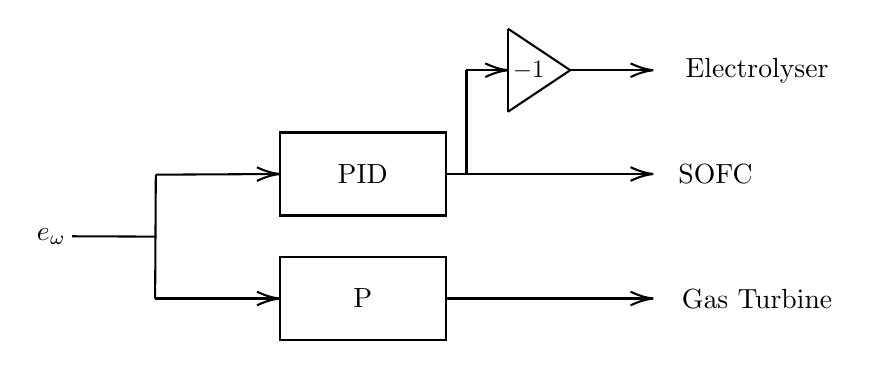
\begin{tikzpicture}[x=0.75pt,y=0.75pt,yscale=-1,xscale=1]
%uncomment if require: \path (0,176); %set diagram left start at 0, and has height of 176
\draw    (127, 56) rectangle (207, 96)   ;
\draw    (127, 116) rectangle (207, 156)   ;

\draw    (67,136) -- (127,136) ;
\draw [shift={(127,136)}, rotate = 180] [color={rgb, 255:red, 0; green, 0; blue, 0 }  ]   (0,0) .. controls (3.31,-0.3) and (6.95,-1.4) .. (10.93,-3.29)(0,0) .. controls (3.31,0.3) and (6.95,1.4) .. (10.93,3.29)   ;
\draw    (67.33,76.33) -- (127,76) ;
\draw [shift={(127,76)}, rotate = 539.6800000000001] [color={rgb, 255:red, 0; green, 0; blue, 0 }  ]   (0,0) .. controls (3.31,-0.3) and (6.95,-1.4) .. (10.93,-3.29)(0,0) .. controls (3.31,0.3) and (6.95,1.4) .. (10.93,3.29)   ;

\draw    (67.33,76.33) -- (67,136) ;


\draw    (27,106) -- (67.17,106.17) ;


\draw    (237,6) -- (267,26) ;


\draw    (207,76) -- (307,76) ;
\draw [shift={(307,76)}, rotate = 180] [color={rgb, 255:red, 0; green, 0; blue, 0 }  ]   (0,0) .. controls (3.31,-0.3) and (6.95,-1.4) .. (10.93,-3.29)(0,0) .. controls (3.31,0.3) and (6.95,1.4) .. (10.93,3.29)   ;

\draw    (207,136) -- (307,136) ;
\draw [shift={(307,136)}, rotate = 180] [color={rgb, 255:red, 0; green, 0; blue, 0 }  ]   (0,0) .. controls (3.31,-0.3) and (6.95,-1.4) .. (10.93,-3.29)(0,0) .. controls (3.31,0.3) and (6.95,1.4) .. (10.93,3.29)   ;

\draw    (237,46) -- (267,26) ;


\draw    (237,6) -- (237,46) ;


\draw    (217,26) -- (237,26) ;
\draw [shift={(237,26)}, rotate = 180] [color={rgb, 255:red, 0; green, 0; blue, 0 }  ]   (0,0) .. controls (3.31,-0.3) and (6.95,-1.4) .. (10.93,-3.29)(0,0) .. controls (3.31,0.3) and (6.95,1.4) .. (10.93,3.29)   ;

\draw    (267,26) -- (307,26) ;
\draw [shift={(307,26)}, rotate = 180] [color={rgb, 255:red, 0; green, 0; blue, 0 }  ]   (0,0) .. controls (3.31,-0.3) and (6.95,-1.4) .. (10.93,-3.29)(0,0) .. controls (3.31,0.3) and (6.95,1.4) .. (10.93,3.29)   ;

\draw    (217,26) -- (217,76) ;



\draw (167,76) node  [align=left] {PID};
\draw (167,136) node  [align=left] {P};
\draw (357,136) node  [align=left] {Gas Turbine};
\draw (17,106) node  [align=left] {$e_{\omega }$};
\draw (337,76) node  [align=left] {SOFC};
\draw (247,26) node [scale=0.9] [align=left] {$-1$};
\draw (357,26) node  [align=left] {Electrolyser};


\end{tikzpicture}
\end{center}
\caption{A diagram to show how PID is used in parallel with proportional control, using the same error signal.}
\label{fig:power-PIDcombo}
\end{figure}